
\chapter%
[Cascade model of memory for multiplication facts]%
{Cascade Model of Memory for Multiplication Facts}

\label{c:xnet}

This chapter describes a connectionist model of memory for multiplication
facts built using \citeauthor{mccascade}'s ``cascade'' equations
\cite{mccascade,pdp3}.  It is referred to as the ``cascade model'' or
``cascade network'' \cite<no relation to cascade correlation,>{cascor}.

The model was originally designed with two objectives in mind. First, in
contrast to the BSB model, the network should be able to capture occasional
errors.  That is, although the network should correctly learn all the
multiplication facts, it should also produce errors when under time
pressure.  The second objective was to minimize the number of assumptions
about connection and unit types.  This objective was formulated in the
context of the \citeA{camp85} model, where many different knowledge
sources were presented.  The aim was to see how many of the assumptions
could be omitted.

The above aims were only selected after it was observed that the
architecture could potentially account for the phenomena.  The network
was first used as
a ``slave'' network, providing arithmetic facts for a
multicolumn arithmetic network---the one described in chapter~\ref{c:fsm},
although the fact network was not used in the final multicolumn network.
The aim was to investigate what kinds of factual knowledge would be useful
to the multicolumn network, hence the same technology was used to build the
fact network (a multilayer perceptron trained with backpropagation).
The results from the work of \citeA{camp85} suggested that the fact network
could be tested for RT and errors. When this was done, a primitive RT
measure showed a dip for 5s problems, prompting further investigation of
the network.

Since then the architecture and representations have changed in many ways.
For example, the first experiments used a one-of-N input encoding and
represented answers in separate tens and units fields.  It was found that
in order to capture human performance, various changes needed to be made.
This chapter first outlines the ``finished product'', after all the changes
have been made. The motivation for the changes, and the results they gave,
are presented in section~\ref{s:variations}.

Much of the literature has focussed on the problems \x22 to \x99.  The
first set of experiments did not simulate ones or zeros problems as human
empirical data had only been found for \x22 to \x99 at that time.  However,
in light of the work of \citeA{harlasso} and \citeA{millcogn}, simulations
of zero and ones problems were performed.  These experiments are presented
in section~\ref{s:01sim}. Finally, the system is compared to the other
connectionist models, and issues arising from the model are discussed.

%-----------------------------------------------------------------------

\begin{fancyfigure}\centerline{%
\psfig{file=xnet.ps,width=12cm,angle=0}}
\caption{Architecture of the cascade model.}
\label{f:xnet}
\end{fancyfigure}

\section{Architecture of the model}

The structure of the network is shown in figure~\ref{f:xnet}. The 17 inputs
to the network are split into two groups of 8 units to encode the presented
digits, 2--9. An additional unit is activated when a tie problem (e.g.,
\x33, \x44) is presented.  The inputs are fully connected to a set of 10
hidden units.  Experimentation showed that 10 hidden units are the
smallest number of units which would reliably learn the problems
in the training set.  That is, networks with less than 10 hidden units would
not always be able to learn the associations.

There is one output unit for each of the products (a one-of-N
``type'' encoding), plus a ``don't
know'' unit (DKU). The tie unit and the DKU are discussed below.  If a
``token'' output encoding was used it would be possible to construct a
model
without hidden units.  This possibility has not been explored.


The two digits that comprise a problem are coarse encoded on the two sets
of input units. Activation falls off exponentially around the presented
digit.  Specifically, the
input to a unit, $u$, for a presented digit, $d$, is given by:
$$ i_{ud} = e^{-0.5(|u-d|/0.85)^2} $$
\noindent where $|u-d|$ is the absolute difference between
$u$ and $d$ (i.e., the distance between the two units).
The constants were arbitrarily chosen so that the digit being encoded
received an input of 1.0, and the
immediate neighbours were 0.5.  Activation continued to
decay beyond the neighbours,
and the input pattern is illustrated here for the digits 5, 6 and 7:
\begin{singlespace}
\begin{verbatim}
    5: 0.00  0.06  0.50  1.00  0.50  0.06  0.00  0.00
    6: 0.00  0.00  0.06  0.50  1.00  0.50  0.06  0.00
    7: 0.00  0.00  0.00  0.06  0.50  1.00  0.50  0.06
\end{verbatim}
\end{singlespace}
\noindent This
choice of representation is discussed in section~\ref{s:variations}.


For adults, tie problems are faster than their position in the
multiplication table would suggest. Although \citeA{siegmult} found a
frequency advantage for tie problems in school textbooks, simulations
suggest (section~\ref{s:presfreq}) that this is not enough to account for
the tie problems' RT advantage.  So for ties an additional input unit (tie
flag) is set to 1.0. Without this, the tie problems were consistently among
the slowest problems for the networks. Hence, the flag is an ad hoc
inclusion which exists only to allow the network to produce faster RTs for
tie problems.
Tie problems are difficult to account for without some change
to the input encoding such as the inclusion of a tie flag.
The information that the two presented digits are equal could be computed
by the network: the problem is the inverse of XOR\@.
The inclusion of a tie flag is making the information
explicit.  The observation here is that the tie flag speeds
response on tie problems. The flag might
be thought of as reflecting the perceptual distinctiveness of tie problems,
possibly as a result of children learning notions like ``same'' and
``different''.


\subsection{Recall}

Networks of the kind described here usually have no reaction time: the
outputs are computed in one step.  A RT measure is implemented in this
system by changing the activation equations.

Once the input units have been set, the ``cascade'' activation equation
\cite[p.~153]{pdp3} is used to simulate the spread of activation in the
network.  The net input to a unit, $i$, at time $t$, is
adjusted to allow activation to build up:
% $$ \net_i(t) = \sum\limits_j w_{ij} a_j(t) + \bias_i $$
$$ \net_i(t) = k \sum\limits_j w_{ij} a_j(t)
+ \bias_i + (1-k)\ \net_i(t-1), $$
\noindent where $w_{ij}$ is the weight between unit $i$ and $j$.
The cascade rate, $k$, determines the rate with which activation
builds up.  It is set to 0.05 in these simulations.  The activity of a
unit is computed with the usual logistic squashing function:
$$ a_i(t) = \frac{1}{1 + e^{-\net_{i}(t)}} $$

\begin{fancyfigure}
\centerline{\psfig{file=cascade.ps,width=9cm}}
\caption{Demonstration of the cascade equations.}
\label{f:cascade}
\end{fancyfigure}

The cascade equations can be thought of as being implemented by a unit with
self-feedback. Figure~\ref{f:cascade} shows how activation builds up with
the cascade
equations.  The net input to a unit determines how fast activation builds
up.  In figure~\ref{f:cascade} the system is simplified and represents a
single unit connected to an input which has a fixed activation of 1.
Variations in the weight produces different activation curves.  The figure
shows the number of iterations required to reach a fixed threshold of 0.7.
 With a large weight of 1.5, 16 iterations are required.
With a smaller weight of 1.0, 37 cycles are needed.  The
activation of the negative
weight decays away.  This example used $k=0.05$:  a smaller value of $k$
would result in more processing steps before the threshold is reached; a
larger value of $k$ would make it more
difficult to discern events that happen in quick succession.

The RT measure is taken to be the number of steps required to reach a
threshold. With a low enough threshold, certain incorrect answers will
reach the threshold. This is not obvious from figure~\ref{f:cascade}, but
is demonstrated below.  Errors tend to be most active early in processing,
although the activation values are often small---typically less than 0.1.
To allow these errors to be accepted, the threshold would have to drop from
a relatively large value, say 0.7, to a small value such as 0.1. Rather
than do this, the output values are normalized. That is, the response of an
output unit is the normalized activation value:
$$ o_i = \frac{a_i}{\sum\limits_j a_j} $$
Here $i$ and $j$ refer to all the output units.
There are a number of ways this normalization could
be implemented in connectionist
terms, but at the moment it is done externally.
Throughout the chapter, and in the figures, this normalized
value is used unless otherwise stated.  To summarize: first the net input
is computed; this is fed into the logistic function to give the activation;
the activation is normalized to give an output signal.  Processing
continues until the activation of a product output unit exceeds a specified
threshold.

To avoid any initial bias towards particular outputs, the activity of the
network is started from a neutral state.  Following \citeA{pdp3}, the
initial state of the network is the state that results from processing an
all-zeros input pattern.  Note that it is not usually enough to start the
system by setting the hidden vector to all zeros: output units may be
selective to the non-activity of certain hidden units.

Originally, the network was trained to turn off all output units when all
the input units are off.  However, it was found this did not quite happen:
certain products were slightly active. These products had an advantage over
the others, and were always more active early in processing---just the
situation that was to be avoided.  This artifact was removed by adding a
``don't know'' unit to the output layer. The network was trained to 
activate only the DKU for an all-zeros input. After training, the DKU had a
positive bias, and all the product units had a negative bias.  The DKU
appears to solve the bias problem, as simulations show that individual
products do not have any advantage over other products. Thus, the DKU is a
computational consideration, and it is not clear what role it might play in
the equivalent human system.  The DKU is not to be confused with subjects
responding ``don't know'' to problems, or omission errors in general.

\subsection{Training}

Two sets of experiments were run.  In the first, the system was trained on
all the problems \x22 to \x99.  The second experiment expanded the
architecture
to
cover \x00 to \x99.  The experiments are described separately below.  In
all cases the problems were trained in a random order using backpropagation
(learning rate 0.01, momentum 0.9).

During training, the presentation frequency of each pattern is skewed in
favour of the smaller problems.
The skew was produced by storing the relative frequency (between zero and
one) of a problem alongside the problem in the training set.  When a
problem was presented to the network, the weight error derivative was
multiplied by the relative frequency value for that pattern. This can be
thought of as providing each input pattern with a different
learning rate. This method allowed accurate control over the presentation
frequencies, without duplicating entries in the training set.

A different skew was used for each of the experiments, but the all-zeros
pattern was always trained with a maximum relative frequency of 1.0.

Although small problems do occur more frequently in textbooks, there is no
reason to believe this skew continues into adulthood
\cite[p.~328]{mcclmode}. To see if the effects of the skew would continue
once the skew was removed, trained networks were further trained on
problems with equal frequencies. That is, in both experiments, two kinds of
networks were produced:  the ``skewed'' networks, which were just trained
on the skewed training set; and the ``equalized'' networks, which resulted
from further training the skewed networks on a training set in which all
problems occurred with equal frequency.

In both experiments, 20 different networks (different initial random
weights) were trained in this way. All results presented below are
mean results taken across the 20 networks.

\citeA{pdp3} note that the asymptotic activation of units under the
cascade equation is the same as that reached after a standard feed-forward
pass. Hence, the network is trained without the cascade equation (with
$k=1$), and then the equation is switched on to monitor the network's
behaviour during recall.

A final detail of the training is that the
derivative of the activation function was
changed slightly. Following \citeA{fahlempi}, a small constant of 0.1 (the
``sigmoid-prime offset'') was
added to the derivative.  Backpropagation
takes the derivative of a unit's activation into consideration when
computing the weights changes.  The derivative of the logistic
activation function is:
$$ f'(a_i) = a_i(1-a_i) $$
\noindent which peaks when the activation of a unit, $a_i$, is 0.5, and
tends towards zero when $a_i$ tends towards 1 or 0.
Intuitively this makes sense: the largest changes should be made to those
units that are ``undecided'', with activations around 0.5.  However, for
some problems the activations may saturate prematurely.
A small derivative slows
learning, and \citeauthor{fahlempi} found that a
network could fail to learn a training set because units had saturated
early on.  Adding a constant to the derivative means that the derivative,
and hence the weight changes, do not get too small when error
remains to be corrected.  Sigmoid-prime offset was found to be essential in
training networks on the multiplication tables, presumably because of the
skew in presentation frequency.

%-----------------------------------------------------------------------

\section{Simulations for \x22 to \x99}\label{s:29sim}

The following experiment was performed to see how well the
model could account for: the RT problem-size effect; exceptions to RT
pattern; and the distribution of operand, close-operand, and table errors.

\subsection{Training}

The 64 problems, \x22 to \x99, were each assigned a frequency according to
the following arbitrary function:
$$ {\rm frequency} = \frac{90-{\rm product}}{88} $$
This produces a linear skew, based on product, in favour of the smaller
problems. For example, \x22 was assigned frequency of 0.96, whereas the
frequency was approximately 0.1 for \x99.
The parameters of this skew were the only ones tested, and the
frequencies are similar to the ones used by \citeA{mcclmath}.  It would
also be possible to explore the effect of basing the skew on a function
other than the product of the two operands. Examples might include the
minimum operand, maximum operand, or sum of operands.  These variations have
not been explored here.

Training on the skewed problems continued to an error
criterion (total sum squared, TSS) of 0.05, taking approximately 8~000
epochs. After this, the networks were trained for a further 20~000 epochs
with equal frequencies reaching a mean TSS of 0.005.  At the end of each
of the training phases, both the ``skewed'' networks and ``equalized''
networks correctly solve all problems.


\begin{fancyfigure}
\centerline{\psfig{file=p3x8.ps,width=13cm}}
\caption{Response of the output units over 40 time steps for the problem
\x38.  Output units representing products over 32 are not shown on this
graph.  The size of each of the squares is proportional to the output of a
particular product unit at a particular moment in processing.}
\label{f:actplot}
\end{fancyfigure}



\subsection{Recall}

On each trial (presentation of a problem) a response
threshold was selected at random from a uniform distribution in
the range 0.4 and 0.9.
Processing then starts from the
all-zeros (``don't know'') state, and proceeds until a product unit exceeds
the threshold. The RT is recorded for a correct
response, and erroneous responses are classified into the categories listed
in chapter~\ref{c:xlit} (e.g., close-operand error, etc).

As the threshold in the recall process is a random element, each problem
must be presented a number of times to capture the mean behaviour of the
networks. Each network is presented with each of the 64 problems 50 times.

Given enough time (usually 50 cascade steps), the networks will produce the
correct response for all 64 problems.  With a high threshold, the network
is allowed this time, and the correct answer is produced.  However, early
in processing erroneous products are active, and with a low threshold these
errors are reported. Presumably the mild time pressure of the experimental
situation results in subjects ``lowering their thresholds''.

For example, figure~\ref{f:actplot} shows the response of a network to the
problem \x38. After the DKU has decayed, the unit representing 27 becomes
active until the network settles into the correct state representing 24.
This is a
demonstration of the operand distance effect, but there is slight
activation of other products: \xeq{3}{7}{21}, \xeq{2}{8}{16},
\xeq{4}{8}{32}, \xeq{3}{3}{9}, and \xeq{2}{7}{14}.

Note that the model predicts that false answers are always recalled more
quickly than correct answers. This is because the false error always
becomes active before the correct one.  Therefore, if it is to be
retrieved, the RT for the incorrect answer will be less than the RT for the
correct answer. \citeA{camp85} only recorded RTs for correct answers, hence
it is not clear that this situation is always the case.  However, it should
be easy to collect evidence to refute or support the model's prediction.
A finding that erroneous RTs are larger than correct RTs is strictly
incompatible with the model as it stands.  Of course other response
mechanisms could be invented.

%For example, processing could start with a
%high threshold which would be lowered in the course of processing.
%Some erroneous responses could have a longer RTs under these conditions.

\begin{fancyfigure}
\centerline{%
\psfig{file=29.ps,height=12cm}}
\caption{Mean correct RT per multiplication table collapsed over
operand order for mean RT of 20 skewed and 20 equalized networks.}
\label{f:rtplottn}
\end{fancyfigure}

\subsection{Results}

The mean RTs of the networks are plotted in figure~\ref{f:rtplottn}. The
RTs show some of the basic features of the problem-size effect, including a
dip for 5s problems.

For the skewed networks the RT correlates $r=0.36$ ($p=0.0018$) with adult
RT \cite{camp85}. This falls to $r=0.19$ ($p=0.063$) after substantial
training on the equalized patterns.  Note that the RTs have reduced and
flattened out for the equalized network, which is just what is expected
after continued practice \cite[p.~349]{camp85}. The obvious feature of the
RT plot is the drop in RT for the nine times table.  Children in grades 3
to~5 respond faster to 9s problems than 8s problems \cite{camp85}, but this
levels out for adults.  The 6s problems are also faster than expected
when compared to human RT\@.
Overall, the skewed network exhibit the best problem-size effect, with
only a slight effect observed on the equalized networks.

The inclusion of a ties unit is necessary to ensure that ties are among the
fastest problems. For the skew networks, the RTs of 6 out of the 8 tie
problems were below the mean RT for their table, increasing to 7 ties for
the equalized networks. \x66 remained above the mean for the six times
table.

\input 29emat.tex

Table~\ref{f:netemattn} shows the error distribution for the 20 networks.
This is similar to the distribution for adults (table~\ref{f:errmat} on
page~\pageref{f:errmat}), although without such a diversity of errors.

Table~\ref{f:errorpc} summarizes the error distribution, and compares them
to \citeauthor{camp85}'s results.  Both sets of networks have error
distributions that are similar to that of adults, but with a larger error
rate. There is little difference between the skewed and equalized networks.

A further point of interest is the correlation between problem error rate
and correct RT. \citeA[p.~110]{camprole} reports a correlation of 0.93 for
adults.  For the skewed and equalized networks $r=0.74$
and $r=0.76$ respectively.  It is not obvious that any model
would necessarily predict that slower problems produce more errors.

The model cannot produce non-table errors as all the output units
correspond to products. \citeA{camp85} report that only 7.4 per cent of
errors are of this kind, so it may not be unreasonable, at first, to focus
on the other errors which make up the majority of the phenomena.
However, non-table errors must be
accounted for, and this topic is taken up in section~\ref{s:xnetdis}.


\def\noteast{\hspace{-1.5em}\mbox{\raise 1mm\hbox{\footnotesize$\ast$}}}
\def\notedag{\mbox{\raise 1mm\hbox{\footnotesize\dag}}}
\setdec 00.0

\begin{fancytable}
\begin{center}
\begin{tabular}{l|cccl}
\multicolumn{1}{c}{}&\multicolumn{2}{c}{Networks}&Adults&\\
&Skewed&Equalized&&\\
\hline
Operand errors          &\dec 90.04 &\dec 86.51 &\dec 79.1 &\\
Close operand errors    &\dec 78.98 &\dec 73.75 &\dec 76.8 &\noteast\\
% Frequent product errors\notedag &\dec 27.76 &\dec 23.68 &\dec 30.6 &\\
Frequent product errors &\dec 25.0 &\dec 20.49 &\dec 24.2 &\\
Table errors            &\dec 9.74  &\dec 13.49 &\dec 13.5 &\\
Operation error         &\dec 3.98  &\dec 3.22  &\dec 1.7 &\noteast\\
Error frequency         &\dec 14.1 &\dec 18.64 &\dec 7.65 &\medskip\\
\multicolumn{1}{l}{\footnotesize$\ast$ Approximate percentage.}\\
%\multicolumn{1}{l}{\footnotesize\dag Percentage of operand errors.}
\end{tabular}
\end{center}
\caption{Percentage breakdown of errors. Figures are mean values from
twenty different networks, and mean values from sixty adult subjects
\protect\cite[appendix.~A]{camp85}.  Note that the model has not been
trained on addition facts, so the frequency of operation errors is
coincidental.}
\label{f:errorpc}
\end{fancytable}


\subsection{Comments}\label{s:09comm}

The following questions are addressed by analysing the trained networks:
\begin{enumerate}
\item Why are certain problems answered more quickly than others?
\item Why are operand errors the most frequent kinds of errors?
\item How are these behaviours established?
\end{enumerate}

RT depends on the net input to a unit, and this can be increased by having
some large, or many small, weights.  The interesting question is why these
weights develop. Presentation frequency, product frequency, initial weight
values, and input encoding are all involved in determining the weights.

The presentation frequency of a problem and product should have a strong
effect on the weights: those problems seen more often should develop larger
weights. Simulations with networks trained on patterns with equal
presentation frequencies alone (section~\ref{s:noskew})
have demonstrated that the frequency of
presentation is important.

However, frequency does not explain why the five times table should be
faster than the four times table. ``Product uniqueness'' may explain why:
none of the products in the five times table occur outside the context of
five (unlike the two times table, where the products 12, 16 and 18 occur in
other tables).  Hence, the error signals for the 5s products are not
diluted through differing hidden representation for different problems.
This explanation is not satisfactory because the same argument should apply
to the seven times table as 7s products are also ``unique''.  The 7s
problems have a lower presentation frequency which may explain the
discrepancy. Also, other simulations which change the product distribution
(e.g., by introducing 10s problems) offer some support for the explanation.
 These simulations are described in section~\ref{s:variations}.

\begin{fancyfigure}
\centerline{\psfig{file=xact.ps,height=12.5cm}}
\caption{Hidden unit activations for one network. Each large rectangle
represents one hidden unit.  Within each rectangle, the size of the smaller
rectangles represents
the activation of the hidden unit to a particular problem. Each large
square mimics the multiplication table (top-left for \x22,
and bottom-right for \x99).}\label{f:xact}
\end{fancyfigure}


In this model the hidden unit encodings are learned (unlike the problem
units in the interactive activation model, or magnitude units in
\citeauthor{camp85}'s model).  The ``receptive fields'' of the hidden units
for one network are plotted in figure~\ref{f:xact}.  Although there are no
dedicated problem units, certain units do respond to sets of problems
(e.g., unit 22 for 3s and 4s problems).  One unit, 21 in this example,
responds to tie problems.  Other units are rather like
\citeauthor{camp85}'s general magnitude units: unit~26 responds to small
products; unit~23 to medium products; and unit~24 responds to larger
products.  The weights between the input layer and the hidden layer are
approximately the same for the two operands.  This is reflected in the
symmetry of the receptive fields.

The hidden units tend to respond to bands of inputs.  This seems to be due
to the coarse coding scheme used for the inputs.  Section~\ref{s:oneofn}
explores this point by looking at the receptive fields that result from a
one-of-N input encoding.
The broad response of the hidden units could be one of
the causes behind the operand distance effect. Hidden units' activities
change smoothly during the course of processing, but at differing rates.
This affects groups of related products due to the overlap in the hidden
encoding (e.g., between unit~23 and 24).  The result is that some
combinations of hidden unit activity may force incorrect
products to exceed threshold.

Other causes for the problem-size effect and operand errors are
discussed in section~\ref{s:variations}.


% -----------------------------------------------------------------------

\begin{fancyfigure}
\centerline{\psfig{file=freq3d.ps,width=6.5cm}}
\caption{Problem frequencies \protect\cite<from>{siegmult}.  The $x$
and $z$ axes represent the multiplication table (rightmost corner
is \x00, leftmost is \x99). The $y$ axis shows the frequency of each
problem.}
\label{f:3dfreq}
\end{fancyfigure}

\section{Simulations for \x00 to \x99}\label{s:01sim}

These simulations were performed for two reasons: first, to see how zero
and ones problems interact with the results from the previous experiments;
and, second, to use more realistic problem frequencies.

\subsection{Training}\label{s:presfreq}

In this experiment the presentation frequencies were skewed according to
the problem frequencies reported by \citeA[table~4]{siegmult}. The
frequencies are shown in figure~\ref{f:3dfreq}, and are derived from the
number of occurrences of each problem in second- and third-grade textbooks.
 These frequency values are, presumably, more ``realistic'' than the
previous skew function that was assumed.  Note, though, that there is a
general decrease in frequency from small to large problems.  Note also the
difference in frequency for zero and ones problems compared to the other
problems.  The contrast to other facts suggests that zeros and ones
problems are treated as different kinds of problem when taught.

To accommodate the extra digits on the input layer, four extra input units
were added---two for each operand to encode zero and one.  The output layer
was increased to cover the extra products that can be produced from zero
and one multipliers.  As the training set was increased from 65 to 101
problems (including the all-zeros pattern), it was found that an extra 2
extra hidden units were required. The network contained 21 inputs, 12
hidden units and 38 output units.

As before, skewed and equalized networks were produced. The skewed networks
were trained for 35~000 epochs to a mean TSS
of 0.07.  A further 35~000 epochs with
equal frequencies were used to produce the equalized networks, reaching a
mean TSS of 0.002.  Again, after training both sets of networks could
correctly recall all the problems.

There was no change to the recall process.

\begin{fancyfigure}
\centerline{\psfig{file=01.ps,height=12cm}}
\caption{Mean correct RT per multiplication table collapsed over
operand order for mean RT of 20 skewed and 20 equalized networks.}
\label{f:rt01}
\end{fancyfigure}


\subsection{Results}

For \x22 to \x99, the results from this experiment are similar to the
previous one. The mean RTs plotted in figure~\ref{f:rt01} show some of the
basic features of the problem-size effect, but these do not appear to be as
good as the RT curves from the previous experiment.
However, for the skewed networks the RT correlates $r=0.22$
($p=0.013$) with adult RT reported by \citeA{millcogn}. This increases to
$r=0.37$ ($p=0.000067$) for the equalized networks. Slightly lower
correlations were found with the \citeA{harlasso} RTs.

The zero problems are solved very quickly.  However, the ones
problems are the among the slowest problems, which is surprising. The 3s
dip is also unexpected.

Again, the RTs have reduced and flattened out for the equalized networks.
Also the 5s and 9s dips
are present, although the dips are comparable to the 3s
dip.  The dip seen for 6s in the previous experiment is not as prominent
here.  All the tie problems were below the mean for their table, except for
\x66. The correlation between RT and error rate was $r=0.74$ for the skewed
networks and $r=0.76$ for the equalized networks.

\setdec 00.0
\def\notedag{\mbox{\raise 1mm\hbox{\footnotesize\dag}}}

\begin{fancytable}
\begin{center}
\begin{tabular}{l|ccc}
\multicolumn{1}{c}{}&\multicolumn{2}{c}{Networks}&Adults\\
&Skewed&Equalized&\\
\hline
Operand errors          &\dec 93.56 &\dec 93.15 &\dec 86.2 \\
Close operand errors    &\dec 78.14 &\dec 74.12 &\dec 76.74 \\
%Frequent product errors\notedag &\dec 22.56 &\dec 20.14 &\dec 26.99 \\
Frequent product errors &\dec 21.11 &\dec 18.76 &\dec 23.26 \\
Table errors            &\dec 6.43  &\dec 6.85  &\dec 13.8 \\
Operation error         &\dec 2.21  &\dec 1.81  &\dec 13.72 \\
%Error frequency         &\dec 10.64 &\dec 15.58 &\dec 6.3 \medskip\\
Error frequency         &\dec 10.64 &\dec 15.58 &\dec 6.3
%\multicolumn{4}{l}{\dag Percentage of operand errors.}
\end{tabular}
\end{center}
\caption{Percentage breakdown of errors. Figures are mean values from
20 different networks, and mean values from 42 adult subjects
\protect\cite[appendix~B]{harlasso}. Adult scores other than
error frequency were recomputed from Harley's data.}
\label{f:err01pc}
\end{fancytable}

A comparison of error types is presented in table~\ref{f:err01pc}.  The
high frequency of operand errors in the ``adult'' column is due to a large
number of errors of the form \xeq{0}{N}{N}.  The network made no errors of
this form---in fact the networks made no errors at all on the zeros
problems.  However, the networks made a number of unrealistic errors by
producing zero as an answer to many problems.  This is shown in
table~\ref{f:netematzn}: the first column shows zero
as an answer for problems such as \x46, \x57 and \x79.

\input 01emat.tex

\subsection{Comments}\label{s:01comments}

This experiment has shown that the speed of the zeros problems can be
accounted for within an associative network. Hence, contrary to various
authors \cite{camp85,millcogn,staznetw}, it is not the RT of zero problems
that suggest zeros are solved by a rule-based mechanism: it is the error
pattern.  Human subjects make errors of the form \xeq{0}{N}{N}.  For the
network, the zero problems were very well-learned, resulting in no errors
on zero problems at all.  However, zero
was unreasonably promoted as an error
for some problems (e.g., \xeq{5}{5}{0}).

It is conceivable that an interaction with addition would change the
system's
behaviour on zero problems.  The introduction of problems such as
0+1=1, 0+2=2, and so on, might have two effects. First, there would no
longer be a simple mapping of ``anything involving a zero is zero'',
reducing the prominence of zero as an unlikely error for some problems.
Second, the addition problems involving a zero may increase the likelihood
of a \xeq{0}{N}{N} error.  On the other hand, the inclusion of addition
problems may increase the RT for zero multiplication problems.  This
speculation should be backed by simulations and
requires more thought (e.g.,
how to incorporate the two operations).

The slow RT of the ones problems may be due to the low frequency of the
problems in the training set.  This seems likely given that the RT for
these problems decreases markedly after further training, as shown for the
equalized networks. However, the ones RT should be comparable to the zeros
problems (cf.\ figure~\ref{f:zerortgraph} on page~\pageref{f:zerortgraph}).
There are numerous ad
hoc ways in which the network could be made to produce
faster RTs for ones problems.
For example, the input representation could be biased towards
zero and ones problems, perhaps by using a logarithmic input encoding, or
just
allocating more input bits to smaller operands. Again, more work is needed
here.


\begin{fancyfigure}
\centerline{\psfig{file=resipsieg.ps,height=9cm}}
\caption{RT derived from the problem frequency shown in
figure~\protect\ref{f:3dfreq}.  The RT is the reciprocal of the mean
frequency of problems in each table.}
\label{f:fake}
\end{fancyfigure}

The change from using a linearly skewed training set to one based on
\citeauthor{siegmult}'s analysis produced a dip in the RT for 3s problems.
This dip can be explained by examining the presentation frequencies: there
is a frequency peak for 3s problems in the training set.  Assuming that RT
is dependent on problem frequency (which is, of course, only part of the
story), it is possible to plot the RT derived from the problem
frequencies.
Figure~\ref{f:fake} is a plot of the reciprocal of mean problem frequency
per table: the idea being that the
more frequent problems require less time to
respond.  The graph clearly shows the 3s dip.  All this suggests that the
networks are heavily affected by changes in problem frequencies.

The presentation frequency also peaks slightly for the five times table.
This may be the reason behind the speed of the fives, but earlier
simulations using a linearly skewed frequency curve also produced the
characteristic 5s dip.

Similar hidden units developed in the two experiments.
Figure~\ref{f:xnetin} displays the net input to each hidden unit for a
network (unlike the previous hidden unit graph, which showed activation).
Unit~27 responds to problems involving a zero, but otherwise the responses
are similar to those for the previous experiment.

\begin{fancyfigure}
\centerline{\psfig{file=wtd01sum.ps,height=11.5cm}}
\caption{Net input to a network's hidden units.  Each large rectangle
represents one hidden unit.  Within each rectangle, the size of the smaller
rectangles represents the net input to the unit for a particular problem.
Negative net input is shown by filled squares, and the size of the square
indicates the magnitude of the net input.}
\label{f:xnetin}
\end{fancyfigure}

%-----------------------------------------------------------------------


\section{Further experiments}\label{s:variations}

The simulations presented above show that the response mechanism produces
errors that are comparable to human errors.  RTs also tend to be faster for
smaller than larger problems, but exceptions to this rule are exhibited.
Some of the causes of this behaviour are discussed below in the context of
variations in the experiments.

\begin{fancyfigure}
\centerline{\psfig{file=oneofn.ps,height=10cm}}
\caption{RTs from simulations of 10 networks trained with a one-of-N input
encoding.}
\label{f:oneofnrt}
\end{fancyfigure}

\subsection{One-of-N input encoding}\label{s:oneofn}

One of the original set of simulations run for the problems \x22 to \x99
used a one-of-N input encoding.  That is, just one input unit was activated
for each operand, rather than using the coarse
encoding.  Other than the change
to input encoding, the rest of the simulation was the same as the \x22 to
\x99 experiments reported above.

Figure~\ref{f:oneofnrt} shows the mean RT from simulations with 10
different skewed networks and 10 equalized networks.  The RT curves
from this experiment were exceptionally good, correlating $r=0.6$ with
the adult RTs reported by \citeA{camp85}.  Note the 7s dip that is expected
from the ``uniqueness'' argument presented in section~\ref{s:09comm}.

The errors were predominantly operand errors (around 97 per cent).
However, only 58 per cent were close-operand errors, compared to 76 per
cent for adults, and only 2 per cent were table errors, compared to 13 per
cent for adults. These observed discrepancies lead to changing the input
representation to the coarse encoding described in previous
experiments.

Note here that the networks trained with the one-of-N
encoding do not need to be trained on false associations to be able to
produce errors. This is in contrast to the
majority of the models described in chapter~\ref{c:xlit}: those models
reply on false associations as a source of errors.
When the input encoding was changed to a coarse encoding the proportion of
close operand and table errors increases.



Previously I have commented \cite{dallmemo} that the cascade model, when
using the coarse encoding, does not
need to be trained on false associations to model the phenomena. Yet, the
coarse coding of operands implicitly introduces false associations. For
example, training on \xeq{5}{8}{40} does not just associate the 5 and 8
input units with the 40 output unit.  Rather, half associations are also
formed between \xeq{4}{8}{40}, \xeq{6}{8}{40}, \xeq{5}{7}{40} and
\xeq{5}{9}{40}.  This is because the 4 and 6, and the 7 and 9 units are
half-activated while the other operand is fully activated. This is, of
course, just the pattern needed to account for close-operand errors (not
operand-errors for \x58, but for the other four problems).  Using the
coarse representation, even smaller associations will be formed for
\xeq{4}{7}{40}, \xeq{4}{9}{40}, \xeq{6}{7}{40} and \xeq{6}{9}{40}.  In this
case both operands are only half-activated, giving a much smaller
association.  This second pattern captures table errors.  It seems, then,
that the change in input encoding introduces false associations which are
suitable for increasing the percentage of close-operand and table errors in
the cascade model.

The input encoding that \citeA{mcclmath} used for MATHNET (a bar of
3 units) should
make all
these false associations with equal strength. Hence it is surprising that
only 5 per cent of MATHNET's
errors were table-errors, and more
errors were non-table errors. The output encoding
for MATHNET consists of tens and units fields, rather than products.  The
interaction between different input
and output encodings may complicate
matters (e.g., input patterns are not attempting to activate particular
products, but are instead activating particular tens and particular units.)

Although the input encoding used by the cascade model (and MATHNET and BSB)
can be conceptualized as a coarseness in the encoding of operands, it can
also be seen as introducing false associations.  The improvements to the
model brought about by introducing a coarse coding could also be effected
by explicitly training on an appropriate set of false products. As such the
model blurs any theoretical difference between the learning of false
associations or the coarseness of operand encoding.  That is, the current
model does not offer a way to choose between the two options, or of
deciding how much each contributes to the phenomena.  Hence in some ways
it does not make sense to ask whether errors are caused by a coarseness in
operand encoding {\em or} by false associations: both produce
false associations.  Deciding if children actually learn false associations
from their environment requires further empirical studies. Likewise,
deciding if children learn false associations as a result of having a
particular kind of operand representation also requires further empirical
studies.

% Ten one-of-n networks
% Skewed:
% Total of 980 errors (tokens),  12.65% of which...
% Operand errors            959.00  97.86%
% Operand distance effect   560.00  57.14%
% High frequency            383.00  39.94%
% Table errors               19.00   1.94%
% Operation errors           50.00   5.10%
%
% Equalized:
% Total of 1497 errors (tokens),  19.32% of which...
% Operand errors           1455.00  97.19%
% Operand distance effect   878.00  58.65%
% High frequency            609.00  41.86%
% Table errors               42.00   2.81%
% Operation errors           56.00   3.74%
%
% Correlations between net and adult RT:
% Campbell     r =   0.60025 p = 0.0

\begin{fancyfigure}
\centerline{\psfig{file=oneofnwts.ps,height=11.5cm}}
\caption{Net input to a network's hidden units with one-of-N input
encoding.
Each large rectangle
represents one hidden unit.  Within each rectangle, the size of the smaller
rectangles represents the net input to the unit for a particular problem.
Negative net input is shown by filled squares, and the size of the square
indicates the magnitude of the net input.}
\label{f:oneofnwts}
\end{fancyfigure}

The receptive field plots that result from a one-of-N input encoding show
some interesting differences to the plots for coarse coding
(figure~\ref{f:oneofnwts}). The encodings
are ``tighter''---they do not show the same degree of broad response that
the coarse encoding produces.  Note also that the hidden units are
responding more selectively for certain tables.  For example: unit~17 is
responding to 6s; unit~18 to 3s; unit~21 to 9s; unit~23 to 7s.

These results indicate that the degree of coarseness (or sharpness) of the
encoding is something that needs to be explored.  The sharpness of the
encoding appears
to play a role in RT (good for sharp, one-of-N encoding),
errors (better with some degree of coarseness) and hidden unit
representations.

\begin{fancyfigure}
\centerline{\psfig{file=noskew.ps,height=12cm}}
\caption{RTs from simulations of 10 networks trained with equal
frequencies only.}
\label{f:noskew}
\end{fancyfigure}

\subsection{Training without a frequency skew}\label{s:noskew}

To assess the importance of the skew in problem frequency, 10 networks were
trained with no frequency skew.  The resulting mean RTs are shown in
figure~\ref{f:noskew}.  Without a frequency skew the RT curve lacks the
problem-size effect.  As expected, then, the skew offers an advantage to
smaller problems.  The figure can be thought of as representing the
inherent difficulty of the input-output mappings in the training set: 3s,
5s and 9s appear to have a natural advantage over other problems.

The coarse input encoding was used, and the errors made by the networks
were mostly operand errors.  Of all trials, 26 per cent resulted in an
error: 87 per cent were operand errors (81 per cent close operand); 25 per
cent were high-frequency errors; 13 per cent were table errors.

% No skew results, 10 networks:
% Total of 2031 errors (tokens),  26.21% of which...
% Operand errors           1777.00  87.49%
% Operand distance effect  1639.00  80.70%
% High frequency            506.00  28.47%
% Table errors              254.00  12.51%
% Operation errors          109.00   5.37%
% Omission errors             0.00   0.00%
% 0xN = N                     0.00   0.00%



\begin{fancyfigure}
\centerline{\psfig{file=mn-rep-rt.ps,height=12cm}}
\caption{RTs from simulations of 20 skewed networks with 12 hidden
units and 20 networks using 20 hidden units.  Both networks used
MATHNET's input representation.}
\label{f:mnsimrt}
\end{fancyfigure}

\subsection{\protect\citeauthor{mcclmath}'s input encoding}

There is a problem with the coarse
input encoding used in the experiments of sections~\ref{s:29sim}
and \ref{s:01sim}: the
encoding is biased against the smallest and largest
operands, favouring the central operands.  The reason is that
the input encoding decays around the operand being encoded, but for the
``edge'' digits (2 and 9, or 0 and 9), there are only neighbours to one
side of the digit.  Hence, other digits (e.g., 5 and 6) supply a larger
input.

The bias towards the central digits may
be one of the reasons why 6s show fast RTs.
The same could be said of 5s
problems, however other simulations show that the effect on 5s is not
significant.  The \x00 to \x99 experiment was re-run using the MATHNET
encoding. Each operand is represented by activating 3 consecutive units
across the 12 input units. The
extra 2 units allow the encoding of 0 and 9
to have activation on both sides.  Hence, no input pattern is favoured,
except for ties which are intentionally favoured.

The results from these simulations are similar, and arguably better, than
the results from the previous input encoding.  Table~\ref{f:mnsimerr}
summarizes the errors, and figure~\ref{f:mnsimrt} shows the RTs.

For this experiment networks with 12 and 20 hidden units were trained.  As
can be seen from table~\ref{f:mnsimerr}, the 20 hidden unit network made
much fewer errors, but all of the errors were operand related.  The 5s dip
vanished for the 20 hidden unit network, but the overall problem-size
effect was
slightly better than the 12 hidden unit network. The 5s dip is prominent
for the 12 hidden unit network, and the 6s dip is absent.  In previous
experiments the 10 and 12 hidden units were used because this was the
smallest number of unit that would reliably learn the training set.
However, these results suggest that the quantity of hidden units is an
important parameter for the model, and the effect of varying the number
should be explored in more detail.

\begin{fancytable}
\begin{center}
\begin{tabular}{l|ccc}
\multicolumn{1}{c}{}&\multicolumn{2}{c}{Skewed nets}&Adults\\
&12 hidden&20 hidden&\\
\hline
Operand errors          &\dec 90.45 &\dec 100.0 &\dec 86.2 \\
Close operand errors    &\dec 82.08 &\dec 98.32 &\dec 76.74 \\
%Frequent product errors\notedag
%                        &\dec 19.98 &\dec 26.62 &\dec 26.99 \\
Frequent product errors &\dec 18.07 &\dec 26.62 &\dec 23.26 \\
Table errors            &\dec 9.55  &\dec 0.0  &\dec 13.8 \\
Operation error         &\dec 1.05  &\dec 0.0  &\dec 13.72 \\
%Error frequency         &\dec 9.51 &\dec 0.83 &\dec 6.3 \medskip\\
Error frequency         &\dec 9.51 &\dec 0.83 &\dec 6.3
%\multicolumn{4}{l}{\dag Percentage of operand errors.}
\end{tabular}
\end{center}
\caption{Percentage breakdown of errors for networks using the MATHNET
encoding.
Figures are mean values from 20 different skewed networks with 12 and 20
hidden units,
and mean values from 42
adult subjects
\protect\cite[appendix~B]{harlasso}. Adult scores other than
error frequency were recomputed from Harley's data.}
\label{f:mnsimerr}
\end{fancytable}


\subsection{Predictions for the 10, 11 and 12 tables}

Children are taught the multiplication tables up to 10, and they were once
taught them up to 12. Out of curiosity, the cascade model was trained on
10, 11 and 12 problems. The input and output layers were expanded to
accommodate the extra numbers, and a total of 15 hidden units were used---a
similar expansion to the one required to model 0s and 1s problems. The
input encoding was the MATHNET encoding described in the previous section.

There are a number of uncertainties with this simulation. First, it is not
clear what kinds of errors or RTs to expect from adults.
Intuition suggests that: 10s
problems will be solved very quickly; 11s problems may
be solved almost as quickly because of the pattern to most of the problems
(for N less than 10, \xeq{11}{N}{NN}, e.g., \xeq{11}{4}{44}); 12s will
probably be the slowest of problems.   A low error rate might be expected
for 10s, a high error rate for 12, and possibly some kind of rule-based
errors could be observed for 11s problems.

Second, it is not obvious that two-digit operands are handled in the same
way as one-digit problems.  Rather than make any more assumptions the 10,
11 and 12 operands are represented in the model in the same way as the
other operands.

Finally, what frequency skew should be used for the extra problems? In this
simulation the \citeauthor{siegmult} skew was used for problems \x00 to
\x99, but a linear skew was used for 10, 11 and 12.
For example, a relative frequency of 0.22 was used for
\x{10}{10}, down to 0.1 for \x{12}{12}.  This was produced by the arbitrary
function:
$$ {\rm frequency} = \frac{180-{\rm product}}{360} $$

Ten skewed and equalized networks were trained under these assumptions. The
resultant error distribution was comparable to previous simulations (95 per
cent operand errors, 73 per cent close-operand, 3 per cent table errors).
No particular patterns were observed. The skewed network produced, on
average, 1.11 per cent of omission errors.  That is, on those trials no
output reached the threshold within 100 cycles.  The equalized networks
produced no omission errors.


The RT graph (figure~\ref{f:predict}) is not unlike the ones reported for
the simulations using the MATHNET input encoding.  The 12s problems are
among the slowest problems, and the 11s problems are solved relatively
quickly, but the 10s are slower than expected.  The graph shows dips for
the primes 3,5,7 and 11, although the 5s dip is not present for the
equalized networks. The disappearance of the 5s dip is perhaps due to the
reduction in ``uniqueness'' of the 5s problems.  The 10s problems interfere
with 5s products, making 5s harder to learn. If 10s really are as easy to
recall as intuition suggests, then the model offers a poor account of 5s
and 10s recall.  This is further discussed later.

A point to note here is that a change in the distribution of products has
changed certain aspects of the RT graph.



% 10 networks trained for the prediction experiment
% Skewed:
% Total of 2695 errors (tokens),  17.97% of which...
% Operand errors           2515.00  93.32%
% Operand distance effect  2004.00  74.36%
% High frequency            607.00  24.14%
% Table errors               70.00   2.60%
% Operation errors           30.00   1.11%
% Omission errors           110.00   4.08%
%
% Equalized:
% Total of 5085 errors (tokens),  33.90% of which...
% Operand errors           4868.00  95.73%
% Operand distance effect  3630.00  71.39%
% High frequency            936.00  19.23%
% Table errors              217.00   4.27%
% Operation errors           22.00   0.43%
% Omission errors             0.00   0.00%

\begin{fancyfigure}
\centerline{\psfig{file=predict.ps,height=12cm}}
\caption{Predictions for 10, 11 and 12 times tables.}
\label{f:predict}
\end{fancyfigure}

%-----------------------------------------------------------------------

\subsection{Damaging the network}\label{s:brainres}

The results from experiments with brain-damaged subjects
\cite<e.g.,>{mcclfact} offer an additional source of findings to compare to
the model.  In this section results are presented from various kinds of
``lesions'' made to trained networks. As described in
section~\ref{s:brainlit}, the main results from the literature include:

\begin{enumerate}
\item Uniform damage for zero problems. That is, the zero problems should
show equal amounts of damage.

\item Nonuniform damage for non-zero problems.

\item Generally, larger problems are more prone to damage.

\item The distribution of errors are similar to the non-damaged
subjects (e.g., errors should be mostly operand errors).

\item There is a close correspondence between complimentary problems.
That is, the
performance on \x46 should be the same as performance on \x64.
\end{enumerate}

There are many ways to damage a network, including: removing units,
altering weights, changing the activation functions, damaging the input
or output units.
The 20 skewed networks from the \x00 to \x99 experiments were
damaged in the following ways:


\begin{fancytable}
\begin{center}
\begin{tabular}{r|rrrrrrrrrr}
&
      0 &   1 &   2 &   3 &   4 &   5 &   6 &   7 &   8 &   9\\
\hline
0 &   0 &  44 &  32 &   0 &   0 &   0 &   0 &   0 &   0 &   0\\
1 &  40 &   0 &   0 &  36 & 100 &   0 &   0 &   0 &   0 &  32\\
2 &   0 &   0 &   0 &   0 &   0 &   0 &   0 & 100 &   0 &  28\\
3 &   0 &   0 &   0 &   0 &   0 &   0 &   0 &   0 & 100 &   0\\
4 &   0 & 100 &   0 &   0 &   0 & 100 &   0 & 100 &   0 &   0\\
5 &   0 &   0 &   0 &   0 &   0 &   0 & 100 &   0 & 100 &   0\\
6 &   0 &   0 &   0 &   0 &  72 & 100 & 100 &   0 &   0 &   0\\
7 &   0 &   0 & 100 &   0 & 100 & 100 &   0 &   0 & 100 &   0\\
8 &   0 &   0 &   0 & 100 &   0 &  96 &   0 & 100 & 100 &  88\\
9 &   0 & 100 & 100 &   0 &   0 & 100 &   0 &   0 &   0 &   0\\
\end{tabular}
\end{center}
\caption{Percentage error on each of the problems \x00 to \x99 for one
network produced with ``relative'' damage.}
\label{f:reldam}
\end{fancytable}



\begin{enumerate}

\item Adding a different random value to all weights
(``absolute'' damage).

\item Multiplying each weight by a different random value (``relative''
damage).

\item Randomly deleting a hidden unit.

\item Reducing the magnitude of the weights by a fixed amount.
\end{enumerate}

Each kind of damage was tried with a variety of parameter settings.
Each network was tested 25 times on each of the 100
problems, with response thresholds randomly selected between 0.8 and 0.9.
This equates to simulations without any time pressure. In all cases damage
resulted in an increase in error rates and in omission errors. None of the
networks produced omission errors before damage.

The values of the parameters of each kind of damage were as follows:
for absolute damage each weight was incremented by a random value between
$\pm1.25$; for relative damage the value was $\pm0.2$; one hidden unit
should be removed; and for magnitude reduction, each weight was reduced by
$1/4$.

Relative and absolute damage gave similar results.  There was no
correlation between error rate and product size. Omission errors occurred on
an average of 37 per cent of trials.
Operand errors and
close-operand errors were prominent, and all errors were nonuniform.  Zero
problems were almost always undamaged. There was little similarity between
complimentary problems.  As an example, the errors resulting from relative
damage for one network are shown in table~\ref{f:reldam}.  The errors
include omission errors.



By deleting a single hidden unit networks could be made to exhibit
non-uniform damage on non-zero problems, and showed a
tendency towards uniform damage for zero
problems. Seven out of 20 networks showed complete uniform damage for
zero problems.
That is, all zeros problems were either 100
per cent correct or 100 per cent incorrect. Six
networks were mostly uniform, with just 2 of the 19 zero problems showing a
different degree of damage.  The other networks were non-uniform on 4, 6 or
8 zero problems. Corresponding problems tended to show the same amount of
damage, as can be seen from table~\ref{f:unitdam}.  In general, there was
no correlation between product size and error rate, and operand errors
varied between 22 and 73 per cent, with a mean of just 45 per cent.
Omission errors also varied greatly, with a mean of 47 per cent of all
errors.

\begin{fancytable}
\begin{center}
\begin{tabular}{r|rrrrrrrrrr}
&
      0 &   1 &   2 &   3 &   4 &   5 &   6 &   7 &   8 &   9\\
\hline
0 & 100 & 100 & 100 & 100 & 100 & 100 & 100 & 100 & 100 & 100\\
1 & 100 & 100 &   0 &   0 &   0 & 100 &   0 &   0 &   0 &   0\\
2 & 100 &   0 &   0 &   0 &   0 &   0 &   0 &   0 & 100 &   0\\
3 & 100 &   0 &   0 &   0 &   0 &   0 &   0 &   0 &   0 &   0\\
4 & 100 &   0 &   0 &   0 &   0 &   0 &   0 &   0 &   0 &   0\\
5 & 100 & 100 &   0 &   0 &   0 &   0 &   0 &   0 &   0 &   0\\
6 & 100 &   0 &   0 &   0 &   0 &   0 & 100 &   0 &   0 &   0\\
7 & 100 &   0 &   0 &   0 &   0 &   0 &   0 & 100 & 100 &   0\\
8 & 100 &   0 & 100 &   0 &   0 &   0 &   0 & 100 &  80 &   0\\
9 & 100 &   0 &   0 &   0 &   0 &   0 &   0 &   0 &   0 &   0\\
\end{tabular}
\end{center}
\caption{Percentage error on each of the problems \x00 to \x99 for one
network produced by removing a hidden unit.}
\label{f:unitdam}
\end{fancytable}

Uniformly reducing the magnitude of weights produced the following effects.
There was a reliable correlation between product-size and error rate, and
damage was non-uniform---including zero problems. Operand errors were
variable, and omission errors were high (around 50 per cent of all errors).
Complimentary problems showed similar error rates.


The results from these simulations are preliminary and inconclusive.  It
seems possible that deletion of just the right hidden unit can produce
uniform errors for zero problems, whilst allowing non-uniform damage on
other problems.  Other kinds of damage show a correlation between the size
of the problem and the number of errors made.  Presumably a mixture of
damage (e.g., some
unit loss and some weight reduction) will be able to produce
the behaviour seen in brain-damaged patients.  However, current simulations
show very high increases in omission errors and a noticeable reduction in
the percentage of operand errors. The reduction in operand errors may not
be serious, as \citeA{mcclfact} report that their patients produced operand
errors on between 35 and 80 per cent of trails.  The large increase in
omission errors may be more important, as 5 out of 7 of
\citeauthor{mcclfact}'s patients showed no omission errors, and the other
two omitted an answer on 46 and 24 per cent of trials (p.~177).

Further simulations are required to clarify these results.  For example, it
may be possible to change the parameters on the methods of damage to reduce
omission errors, or just lower the response threshold.  The general problem
here is that there are many parameters to consider: not only parameters to
the methods of damaging networks, but different ways to damage networks.
There also appear to be no good reasons for choosing one kind of damage
over another, or indeed, for supposing that one kind of damage simulates
the damage suffered by patients.

For these experiments mean results are not generally useful.  This creates
a problem because one cannot easily be certain that an observed pattern of
damage is typical and reliable, or just an artifact of a
particular parameter setting. Rather than report mean statistics, it is
necessary to classify each network in some way.  It is not obvious how to
form these categories, but they might include some kind of error
rate uniformity measures for each table. More work is required before this
aspect of the model can be systematically explored. It is nevertheless
encouraging to see that non-uniform errors can be produced, and that there
is some potential for producing uniform errors for zero problems.


%-----------------------------------------------------------------------

\section{Discussion}\label{s:xnetdis}

The preceding simulations and analysis have suggested the following causes
for the problem-size effect and operand errors:

\begin{itemize}

\item {\em The
input encoding.}  Presented digits are associated with all the
products in the digit's table, producing operand errors.  Close-operand
errors result from false associations formed by the coarseness of the input
encoding.

\item {\em The presentation frequency.}
Smaller problems are presented more
often than larger problems, and this is the foundation of the problem-size
effect.

\item {\em The
nature of the facts themselves.} Certain problems, such as 5s, may
be easier to learn due to the distribution of the associated products. That
is, 5s products
participate only in problems involving the digit 5, unlike,
say 6s products, which are found in problems where a 6 is not a presented
operand. This effect may be enhanced or reduced by the choice of output
encoding, or more generally speaking, by the details of the input-output
mapping to be learned in the context of the recall architecture.

\end{itemize}


The simulations have shown that the model is affected by these parameters.
The change from a one-of-N input encoding to a coarse encoding changed the
simulation results.  Changes in presentation frequency were not explicitly
explored,
and were compounded with changes to the problem set brought about by the
introduction of zero and ones problems.  The distribution of products was
modified with the introduction of 10s, 11s and 12s problems.  This brought
about a change in the RT results.  Future work should look at how
systematic changes to these parameters change the performance of the model.

Some of the general issues that arise from the model are discussed below.
The next section looks at the choice of output representation.
Section~\ref{s:rulesres} discusses the problems posed by the zero and ones
problems. Section~\ref{s:verifyres} speculates as to how verification and
primed production tasks could be incorporated into the model.


\subsection{Choice of output representation}

Non-table errors are not accounted for because the outputs of the model are
represented as product nodes.  This choice has a number of consequences.
First, it means that a separate read-out mechanism is required to capture
non-table errors.  One possible scheme would be to add a tens layer and a
units layer above the product layer in the network.  The details of this
scheme have not been worked out, but one could imagine that the system
would be similar to the current model.  Each unit or ten node would receive
a different number of connections from the product nodes. For example, the
tens unit representing 60, would be connected to 2 products (64 and
63), whereas the 70s unit would receive input from just the 72 product. In
this way, each of the tens and units nodes would show differing RTs and
error rates. Whether this system produces non-table errors while preserving the
distribution of the other types of error remains to be seen.  Note, though,
that the scheme brings added complexity: is RT measured when either the
tens of units fields exceed a threshold, or both?  Does the read-out
mechanism operate in parallel with the rest of the system, or is it
used after a product unit exceeds threshold?

Results from the work of \citeA[pp.~99-108]{harlasso} support the
plausibility of a separate read-out mechanism. \citeauthor{harlasso}'s
experiments measured the table-error rates of subjects solving
multiplication problems, and the error rates for just reading numbers. The
analysis of the results suggested that non-table errors occurred in 0.14 per
cent of reading trials.  Multiplication produces 0.52 per cent non-table
errors.  This is not a statistically significant difference in error rates.
As such there is no reason to reject the null hypothesis that non-table
errors from reading and recall result from the same mechanism.  Presumably
this shared mechanism is not part of fact recall, and is more likely to be
part of some kind of read-out mechanism---the number production element
of the modular structure of number processing shown in
figure~\ref{f:numstruct}. To pursue this argument further
requires the specification of an explicit read-out mechanism.  This aspect
of the model is an avenue for future study.

A second point of interest surrounds the formation of product units.
It is not unreasonable to suppose that certain, often encountered, numbers
are represented as single nodes.  However, there are limits to this
representation, but it is not obvious what these limits are.  At some
stage a more general ``parsing'' mechanism may be employed to handle
longer numbers, and it may even be related to the read-out mechanism.
It is assumed here that memory for simple arithmetic facts is a
modular system, but at some stage the connection between product units and
other representation of number should be explored.

The cascade model does not attempt to explain the formation of product
units, and simply assumes that product units are pre-formed.  How and why
certain numbers are represented in this way is one of the many
questions not addressed here.

%-----------------------------------------------------------------------

\subsection{Rule based processing}\label{s:rulesres}

Error results from normal and brain-damaged subjects indicate that zero
and ones problems are not handled in the same way as other multiplication
facts.  To recap, RTs for zero and ones problems are low, and zero errors
tend to be of the form \xeq{0}{N}{N}.  Brain-damaged subjects show uniform
impairment on zeros problems, and recover the ability to solve zero
problems after  remediation on just two zero problems.  The cascade model,
although fast on zero problems, is not fast on ones problems, and pays a
penalty of offering zero as an answer to many problems.

Section~\ref{s:01comments} speculated as to how the model could be modified
to account for these findings.  Specifically, it was suggested that the
introduction of addition would reduce the strength of zero associations and
offer the possibility of \xeq{0}{N}{N} errors. This suggestion is hard to
evaluate as no accounts have been given of how addition and multiplication
interact.

The suggestion of a separate mechanism, presumably using rules, for 0 and
1, is not without problems (section~\ref{s:ruleslit}), but is attractive.
The results from the cascade model, for example, are best when zero and one
problems are excluded. No models have been offered to explain how such a
dual-process account would work, and the task of building such a model
seems large.
Rather than do this, I suggest first further exploring the models we have.
In particular, the mixing of addition with multiplication has been left
almost untouched. Yet children learn multiplication only after learning
addition, and addition appears to fuel zero and one errors. I propose the
interactions between the two operations should be explored before separate
mechanisms for certain operands are suggested.


%-----------------------------------------------------------------------


\begin{fancyfigure}
\centerline{\psfig{file=poss-verify.ps,width=13cm}}
\caption{Possible account of verification for the cascade model.}
\label{f:possverify}
\end{fancyfigure}

%-----------------------------------------------------------------------
\subsection{Verification and primed production tasks}\label{s:verifyres}

The settling models (IA, BSB, MATHNET) appear better suited to verification
and priming tasks than the cascade model.  The typical verification account
(e.g., from BSB and IA) involves clamping input and output units and
measuring the time required to reject or accept the suggested product. This
apparently straight-forward way to model verification has a number of
problems.  First, it is necessary to only slightly activate the output
layer.  If the product to be tested was presented with full activation,
surely the response mechanism should respond with that product immediately.
The alternative is to delay the response in some way, but this has not been
suggested by any of the models. It is not clear why the output layer should
receive less activation from the presented problem than the inputs do. The
motivation for this assumption is not clear from the IA account, and the
BSB account does not clarify what assumptions it makes about product
priming.

Figure~\ref{f:possverify} sketches one way in which the cascade model could
be changed to capture verification.  This speculative suggestion
involves adding a separate network to the existing recall network.
The verification network is presented with a product, while the recall
network is presented with the two operands as usual. The hidden layer of
the
recall network forms part of the input to the verification network, and
this should
allow the system to verify the presented product.  Note that a shared
representation is presumed because it seems wasteful to suppose that the
verification network requires a completely independent fact store.

The details of the verification system and the coupling to the recall
network have not been worked out.  For example, it is not clear how or why
the verification network is trained, or if the training aids the recall
network.  Nor is it clear how control is allocated between the networks.
However, it predicts that the verification network can be damaged, whilst
the recall network remains intact. If the weights between the hidden layer
and output layer of the recall network were independently damaged, it is
possible that verification could proceed while production fails.

There is little evidence to support or refute the idea of verification
process that is, in some interesting sense, separate from the recall
process. However, tentative support comes from the study of a single
brain-damaged subject by \citeA{dageorga}. The subject was much better on
the production task for subtraction than addition or multiplication.
However, performance was comparable on all three operations for the
verification task. \citeauthor{dageorga} ``\ldots suggest that the
production/verification differences may be taken as support for the view
that arithmetic fact retrieval processes are not the same in production and
verification tasks'' (p.~20).

Support for a separate mechanism presents a second problem for the settling
models' account of verification.  As verification is perceived as the
product of a bidirectional settling process, why should damage selectively
alter performance on just verification or just production? For the cascade
model, a separate mechanism seems necessary to even begin simulations of
the verification task.


\begin{fancyfigure}
\centerline{\psfig{file=chain1.ps,width=13cm,height=7cm}}
\caption{\x84 followed by \x68.}
\label{f:chain1}
\end{fancyfigure}

Primed production is not so easy to model with the cascade system. The task
requires some way to prime particular products before a problem is
presented.  Although output units could be activated before recall, it is
not clear how this can be done without triggering the response mechanism
(as described above). However, it is possible to show that the cascade
model is sensitive to the context in which a problem is presented.  In
figure~\ref{f:chain1}, the system has been presented with \x84.  After 40
processing cycles the input was changed to \x68 without resetting the
network to the ``don't know'' state. The vertical line in the centre of the
figure shows the point at which the input was changed.  The network
required 40 steps to reach threshold for the problem \x68, stepping up
through the 8 times table to reach the correct product.

Now consider figure~\ref{f:chain2}.  Here the first problem was \x33, and
the second remained at \x68.  The simulation shows clear differences in the
processing, and 49 steps were required for an output unit to reach
threshold on the \x68 problem.  The simulation had to ignore the fact that
the previous product was above threshold when processing of the next
problem began.  This difficulty may be avoided if it is assumed that the
activity of the system decays, to some degree, towards the zero-state
before another product is presented.

These simulations also suggest a way for the model to produce different
responses for a particular problem. Previous simulations have been
deterministic:  the response to a particular problem is always the
same after training is complete.  This is, in part, because the state of
the system is reset at the start of processing to the ``don't know'' state.
If the system is not reset, different responses will
be produced.  This context sensitivity is another possibility to be
pursued.


\begin{fancyfigure}
\centerline{\psfig{file=chain2.ps,width=13cm,height=7cm}}
\caption{\x33 followed by \x68.}
\label{f:chain2}
\end{fancyfigure}


%-----------------------------------------------------------------------

\section{Summary}

The cascade model can capture aspects of RTs and errors of adults recalling
multiplication facts.  This chapter has outlined the assumptions required
to do this, including assumptions about problem frequency and input
representation.  An initial analysis of the system has been presented, and
variations on the model have been explored in an attempt to identify the
factors that determine the behaviour of the system.  In addition,
simulations have been run to address the issue of zero and ones
problems, and of network damage.

The cascade model requires further work:
\begin{itemize}
\item The RT results could better match the human results.  With a one-of-N
encoding, good RT curves are produced, but the errors are not so well
distributed.
\item Tie problems are solved by an ad hoc inclusion of a tie flag.
\item The model does not capture the phenomena associated with zero
and ones problems.
\item Non-table errors are not explained.
\item The verification and primed-production tasks are not accounted for.
\end{itemize}

However, an attempt has been made to present an explicit set of simulations
that can be easily appraised.  This is in contrast to other poorly-specified
connectionist models, with the exception of MATHNET\@.  Construction of the
model has lead to a number of suggestions, in particular concerning the
nature of false associations and coarse encoding, and of the verification
task and zero and ones problems.

All of the connectionist models discussed use differing methods to measure
RT, different input or output representations, different learning rules,
training sets, hidden units, and so on, yet all show some degree of match
to human behaviour.  It seems that any kind of associative structure, with
appropriate parameter settings, will fit the human empirical phenomena.
This is encouraging because it seems that associative networks are just the
right tools to model arithmetic fact recall.  It is also discouraging
because it hampers the discovery of the features that are responsible for
determining the behaviour of human systems.

Plenty of important differences exist between the systems. The
continued development of each of the models holds the promise of
identifying those aspects that are pertinent to understanding human
multiplication abilities---and weeding out those that are not.

As mentioned above, the cascade, MATHNET and IA models have been
developed independently. One useful direction for this work is to look at
the assumptions of the other models, and to see how they effect the
performance of the cascade system.  This could be profitable for
discovering combinations of features that are sufficient to account for
human behaviour. For example, although a tens and units
output representation was originally used in the cascade model, it did not
capture the distribution of errors found for adults.  However, the model
has developed since then, and it could be that the negative result was due
to other parameters, such as the input representation.  On the other hand,
the representation of products may be a necessary feature of the model.

Throughout the chapter various ideas have been proposed as directions for
future work. Some of the quickest extensions to the model include: adding a
tens and units read out mechanism; detailing and training the verification
network; testing the effect of various parameters, such as the number of
hidden units or training times. Longer term goals include: exploring the
relationship between addition and multiplication; studies of the effect of
changes to the input representation, such as logarithmic input encodings;
studies of pre-multiplication number understanding; systematic studies of
network damage. However, the most pressing need is for a further
systematic analysis of the existing networks: why are 9s so easy to recall?
What are the effects of changes to problem frequency?  What happens to the
network as the weights develop during training? What are the effects of
changes to the distribution of products?  How would systematic changes to
the sharpness of the input encoding alter the results?
An
understanding of the influences
that lead to successful models may help develop an understanding of human
arithmetic skills.
